\section{Definitions}
%\subsection{Definitions}
\textbf{Edge coloring:} 
\textit{``An edge coloring of a graph G is a coloring of the edges of G in such a way that two edges which share a vertex have different colors."}
\\[0.5cm]
\textbf{Chromatic index:}
\textit{``The chromatic index of a graph G, denoted by ${\chi'(G)}$ is the minimum number of colors necessary for the edge-coloring of G."}
\\[0.5cm]
The maximum degree of a graph G is denoted by $\Delta(G)$. For any graph $G$, $\chi'(G) \geq \Delta(G)$. It means that all the edges around a vertex with degree $\Delta(G)$ must have different colors.
\\\\
\textbf{Vizing's theorem}$^{\cite{berge1991short}}$
\textit{``For any graph $G$, $\chi'(G) \leq \Delta(G) + 1$"}.
\\
Thus the only possible values for $\chi'(G)$ are $\Delta(G)$ or $\Delta(G)+ 1$.\\
To prove the Vizing's theorem, we use "A constructive proof of the theorem of Vizing"$^{\cite{misra1992constructive}}$ to obtain a $\Delta(G)+ 1$ edge-coloring for graphs.\\[0.5cm]
\textbf{The fan}$^{\cite{misra1992constructive}}$~\\
They defined a data structure called ``fan". A fan $<f..l>$ of X (X is a vertex), is a sequence of vertices that satisfies the following properties:
\begin{itemize}
\item F0: $<f..l>$ is a nonempty sequence of distinct neighbors of X
\item F1: edge Xf is uncolored (the other edges of the fan are colored)
\item F2: ($\forall$ u:: color of edge $Xu^+$ is free at u ($u^+$ is the successor of u in the fan))
\end{itemize}
For example, on the graph below (see figure \ref{fig:fan}). Edge AB is not colored (dashed line) and another edges are coloring. A fan $F1= \{ B, D, C\}$ of A is maximal fan. And $F2 = \{ B, C\}$ is another fan of A but it is not maximal.
\\
\begin{figure}[h!]
\centering
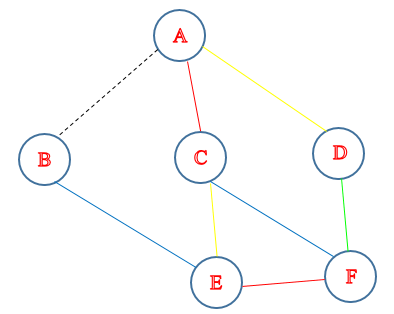
\includegraphics[width=0.4\textwidth]{./images/fan}
\caption{Graph with a edge uncolored}
\label{fig:fan}
\end{figure}
\\[0.5cm]
\textbf{Inverting a path}$^{\cite{misra1992constructive}}$~\\
A cd-path of X is a path that includes vertex X, has edges colored only c or d, and is to be maximal.
The operation ``invert the cd-path" switches every edge on the path colored c to d and vice versa.\\
As above example (figure \ref{fig:fan}), $ \{AD, DF\}$ is a yellow-green path of A. And after invert, the its color change from yellow to green and vice versa. As the followed result (see figure \ref{fig:fan_invert}). \\
\begin{figure}[h!]
\centering
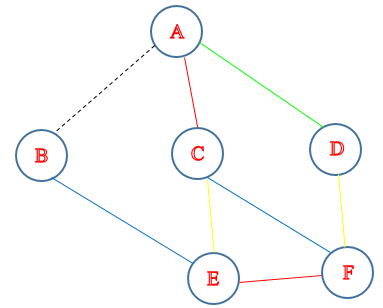
\includegraphics[width=0.35\textwidth]{./images/fan_invert}
\caption{Graph after inversion the yellow-green path of A}
\label{fig:fan_invert}
\end{figure}~\\
\textbf{Rotating a fan}$^{\cite{misra1992constructive}}$~\\
Given a fan $F[1:k]$ of a vertex X, the ``rotate fan" operation does the following in parallel:
\begin{itemize}
\item $c(F[i],X) = c(F[i+1],X)$
\item Uncolor $F[k]$
\end{itemize}
This operation leaves the coloring valid, as for each i, $c(F[i+1],X)$ was free on $(F[i],X)$.\\\\
With the graph in figure \ref{fig:fan_invert}, we can easy find a fan of A: $F=\{B,C,D \}$. We apply the rotation on fan $F$. The result change the color of fan-edge as bellow image (see figure \ref{fig:fan_rotation}).\\
\begin{figure}[h!]
\centering
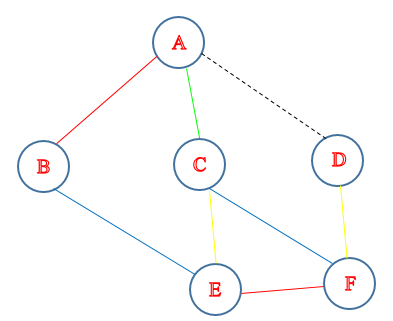
\includegraphics[width=0.3\textwidth]{./images/fan_rotation}
\caption{Graph G after rotation a fan $F=\{B, C, D\}$}
\label{fig:fan_rotation}
\end{figure}~\\\\
\textbf{The algorithm}$^{\cite{misra1992constructive}}$~\\
\begin{algorithm}[H]
\KwData{A graph G}
\KwResult{A proper coloring c of the edges of G}
Let $U:=E(G)$\\
\While{U is not empty}{
\begin{enumerate}
\item Let $(u,v)$ be any edge in U
\item Let $F[1:k]$ be a maximal fan of u starting at $F[1]=v$
\item Let $c$ be a color that is free on $u$ and $d$ be a color that is free on $F[k]$
\item Invert the $cd_u$ path
\item Let $w \in V(G)$ be such that $w \in F, F^{'}=[F[1]..w]$ is a fan and d is free on $w$
\item Rotate $F^{'}$ and set $c(v,w)=d$
\item $U:=U-\{(u,v)\}$
\end{enumerate}
}
\end{algorithm}
\textbf{Proof}: Refer to \cite{berge1991short}.\\\\
The following example illustrate the algorithm. A graph with four vertices $(A, B, C, D)$ and five edges including two edges are not coloring $(AC, BD)$ and another edges are coloring (figure \ref{fig:graph_ex1}).\\
To reduce the time execution algorithm, we only consider the un-colored edges. So, the set of edges is $U=\{AC, BD\}$.\\
The round 1: consider $AC$ edge.
\begin{itemize}
\item Maximal fan of $A$: $F=\{C\}$ (because blue not free on C)
\item Color c is free on $A$, and color d is free on $C$. We choose $ c $ is red and $ d $ is yellow (because both red and blue are not free on C). The red-yellow path of A is empty.
\item We choose $w = C$ because the fan $F$ has only one member. 
\item Set the color of $AC$ is yellow. The set $U=\{BD\}$
\end{itemize}~\\
\begin{figure}[h!]
\centering
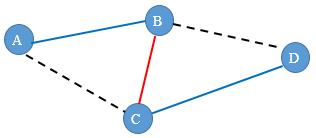
\includegraphics[width=0.3\textwidth]{./images/graph_ex1}
\caption{Graph G }
\label{fig:graph_ex1}
\end{figure}~\\
After round 1, $AC$ colored and the graph is following:\\ 
\begin{figure}[h!]
\centering
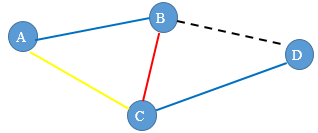
\includegraphics[width=0.3\textwidth]{./images/graph_ex2}
\caption{Graph G after AC colored by yellow}
\label{fig:graph_ex2}
\end{figure}~\\
The round 2, consider $BD$ edge:
\begin{itemize}
\item Maximal fan of $B$: $F=\{D,C\}$ (because blue not free on A and C)
\item Color c is free on $B$, and color d is free on $C$. We choose $ c $ is yellow and $ d $ is green (because both red, blue and yellow are not free on C). The yellow-green path of B is empty.
\item We choose $w = C$ because no fan edge has color green. The new fan is also F: $F_1 = F = \{D,C\}$
\item Rotate fan $F_1$ (figure \ref{fig:graph_ex3}) and color BC by green (figure \ref{fig:graph_ex4}). The set $U=empty$
\end{itemize}~\\

\begin{figure}[h!]
\centering
\subfloat[Graph G after rotation the fan $F_1$]{\label{fig:graph_ex3}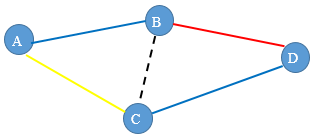
\includegraphics[width=0.35\textwidth]{./images/graph_ex3}}~~
\subfloat[Graph G after BD colored by green]{\label{fig:graph_ex4}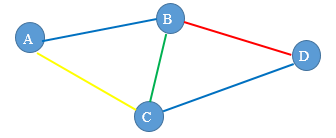
\includegraphics[width=0.35\textwidth]{./images/graph_ex4}}
\caption{The graph was colored after execute the edge coloring algorithm}
\label{fig:graph_ex5}
\end{figure}~\\
The algorithm stopped by the set $U$ empty.
%\subsection{Objectives}
%Objectives...\ref{intro}
\section{Specifications}
The crucial requirement of our program is to visualize the graph's algorithms. The input does not contain any information for the graph in the GUI. The program allows the user to display the graph on the GUI which follows the style coding conventions defined by the programmer. The vertices are represented by the labeled circles. The transitions are represented by the straight lines, it also displays the labels for transitions.
\\[0.5cm]
This application represents the graph on the circle model. Depend on the number of vertices, program automatically defines the position of each vertex.
\\[0.5cm]
Program allows the users to run the breadth-first search on the GUI. The vertices automatically change its colors when program executes on it (push, pop a vertex). Besides, it also changes the color of edge to display the BFS tree.
\\[0.5cm]
At last, the application implements the Misra and Gries edge coloring algorithm. It calculates the number of colors to color the edges of graph and coloring it.